\begin{frame}{Classification Task}
    \begin{definitionblock}{Definition}
        \centering
        \begin{itemize}
            \item<1-> Dataset $\mathcal{D}$: set of input-output pairs
            \[
                \mathcal{D} = {\{(\mathbf{x}_i, y_i)\}}_{i=1}^n\,,
            \]
            where $\mathbf{x}_i \in \mathcal{X}$ is an input vector and $y_i\in \mathcal{Y} = \{c_1, \dots, c_K\}$ is its corresponding label;
            \item<2-> $y_i$ can be transformed into vector form $\mathbf{y}_i\in \mathcal{Y} = {\{0,1\}}^K$ using one-hot encoding:
            \[
                y_{ij} = 
                \begin{cases}
                    1, \text{if $\mathbf{x}_i$ has label $c_j$}\\
                    0, \text{otherwise}\,.
                \end{cases}
            \]
        \end{itemize}
    \end{definitionblock}
\end{frame}

\begin{frame}{Classification Task}
    \begin{definitionblock}{Definitions}
        \centering
        \begin{itemize}
            \item<1-> Underlying mapping $f$: a function
            \[
                f:\mathcal{X} \to \mathcal{Y}
            \]
            that maps input vectors to output labels.
        \end{itemize}
    \end{definitionblock}
\end{frame}

\begin{frame}{Classification Task}
    \begin{normalblock}{Classification aim}
        \centering
        \begin{itemize}
            \item<1-> Given input $\mathbf{x}_i$, aim is to correctly predict label $\mathbf{y}_i$.
            \item<2-> Training process: $f$ is approximated using a parametrized function $f_{\theta}$:
            \[
                f_{\theta}: \mathcal{X} \to \mathcal{Y}\;,
            \]
            that minimizes the \emph{empirical risk}: 
            \[
                \mathcal{R}_{\epsilon}(\theta) \coloneqq \frac{1}{n}\sum_{i=1}^{n} L(\mathbf{y}_i,f_{\theta}(\mathbf{x_i}))\,.
            \]
        \end{itemize}
    \end{normalblock}
\end{frame}

\begin{frame}{Loss Function}
    \begin{definitionblock}{Definition}
        \centering
        \begin{itemize}
            \item<1-> Loss function $L$: measures the dissimilarity between predicted and true labels.
            \item<2-> Different possibilities:
            \begin{align*}
                L_{0, 1} &= \frac{1}{n} \sum_{i=1}^{n} \mathbb{I}(y_i, f_{\theta}(\mathbf{x}_i))\\
                L_{RMSE} &= \frac{1}{n}\sqrt{\sum_{i=1}^{n} {(y_i-f_{\theta}(\mathbf{x}_i))}^2}   
            \end{align*}
        \end{itemize}
    \end{definitionblock}
\end{frame}

\begin{frame}{Artificial Neural Network}
    \begin{figure}
        \centering
        \scalebox{0.7}{
        \begin{tikzpicture}[x=3cm,y=1.2cm]
            \message{^^JNeural network, shifted}
            \readlist\Nnod{4,5,5,5,3} % array of number of nodes per layer
            \readlist\Nstr{n,m,m,m,k} % array of string number of nodes per layer
            \readlist\Cstr{\strut x,a^{(\prev)},a^{(\prev)},a^{(\prev)},y} % array of coefficient symbol per layer
            \def\yshift{0.5} % shift last node for dots
            
            \message{^^J  Layer}
            \foreachitem \N \in \Nnod{ % loop over layers
            \def\lay{\Ncnt} % alias of index of current layer
            \pgfmathsetmacro\prev{int(\Ncnt-1)} % number of previous layer
            \message{\lay,}
            \foreach \i [evaluate={\c=int(\i==\N); \y=\N/2-\i-\c*\yshift;
                        \index=(\i<\N?int(\i):"\Nstr[\lay]");
                        \x=\lay; \n=\nstyle;}] in {1,...,\N}{ % loop over nodes
                % NODES
                \node[node \n] (N\lay-\i) at (\x,\y) {$\Cstr[\lay]_{\index}$};
                
                % CONNECTIONS
                \ifnum\lay>1 % connect to previous layer
                \foreach \j in {1,...,\Nnod[\prev]}{ % loop over nodes in previous layer
                    \draw[connect,white,line width=1.2] (N\prev-\j) -- (N\lay-\i);
                    \draw[connect] (N\prev-\j) -- (N\lay-\i);
                    %\draw[connect] (N\prev-\j.0) -- (N\lay-\i.180); % connect to left
                }
                \fi % else: nothing to connect first layer
                
            }
            \path (N\lay-\N) --++ (0,1+\yshift) node[midway,scale=1.5] {$\vdots$};
            }
            
            % LABELS
            \node[above=0.4,align=center,mygreen!60!black] at (N1-1.90) {input\\[-0.2em]layer};
            \node[above=0.1,align=center,myblue!60!black] at (N3-1.90) {hidden layers};
            \node[above=0.85,align=center,myred!60!black] at (N\Nnodlen-1.90) {output\\[-0.2em]layer};
            
        \end{tikzpicture}
        }
        \caption*{Feedforward neural network}
    \end{figure}
\end{frame}

\begin{frame}{Convolutional Neural Network}
    \begin{figure}
        \centering
        \scalebox{0.7}{
            \begin{tikzpicture}[x=1.6cm,y=1.1cm]
                \large
                \message{^^JDeep convolution neural network}
                \readlist\Nnod{5,5,4,3,2,4,4,3} % array of number of nodes per layer
                \def\NC{6} % number of convolutional layers
                \def\nstyle{int(\lay<\Nnodlen?(\lay<\NC?min(2,\lay):3):4)} % map layer number on 1, 2, or 3
                \tikzset{ % node styles, numbered for easy mapping with \nstyle
                  node 1/.style={node in},
                  node 2/.style={node convol},
                  node 3/.style={node hidden},
                  node 4/.style={node out},
                }
                
                % TRAPEZIA
                \draw[visible on=<3->, myorange!40,fill=myorange,fill opacity=0.02,rounded corners=2]
                  %(1.6,-2.5) rectangle (4.4,2.5);
                  (1.6,-2.7) --++ (0,5.4) --++ (3.8,-1.9) --++ (0,-1.6) -- cycle;
                \draw[visible on=<2->, myblue!40,fill=myblue,fill opacity=0.02,rounded corners=2]
                  (5.6,-2.0) rectangle++ (1.8,4.0);
                \node[right=19,above=1.05,align=center,myorange!60!black] at (3.1,1.8) {convolutional\\[-0.2em]layers};
                \node[above=1,align=center,myblue!60!black] at (6.5,1.9) {fully-connected\\[-0.2em]hidden layers};
                
                \message{^^J  Layer}
                \foreachitem \N \in \Nnod{ % loop over layers
                  \def\lay{\Ncnt} % alias of index of current layer
                  \pgfmathsetmacro\prev{int(\Ncnt-1)} % number of previous layer
                  %\pgfmathsetmacro\Nprev{\Nnod[\prev]} % array of number of nodes in previous layer
                  \message{\lay,}
                  \foreach \i [evaluate={\y=\N/2-\i+0.5; \x=\lay; \n=\nstyle;}] in {1,...,\N}{ % loop over nodes
                    %\message{^^J  Layer \lay, node \i}
                    
                    % NODES
                    \node[node \n,outer sep=0.6] (N\lay-\i) at (\x,\y) {};
                    
                    % CONNECTIONS
                    \ifnum\lay>1 % connect to previous layer
                      \ifnum\lay<\NC % convolutional layers
                        \foreach \j [evaluate={\jprev=int(\i-\j); \cconv=int(\Nnod[\prev]>\N); \ctwo=(\cconv&&\j>0);
                                     \c=int((\jprev<1||\jprev>\Nnod[\prev]||\ctwo)?0:1);}]
                                     in {-1,0,1}{
                          \ifnum\c=1
                            \ifnum\cconv=0
                              \draw[connect,white,line width=1.2] (N\prev-\jprev) -- (N\lay-\i);
                            \fi
                            \draw[connect] (N\prev-\jprev) -- (N\lay-\i);
                          \fi
                        }
                        
                      \else % fully connected layers
                        \foreach \j in {1,...,\Nnod[\prev]}{ % loop over nodes in previous layer
                          \draw[connect,white,line width=1.2] (N\prev-\j) -- (N\lay-\i);
                          \draw[connect] (N\prev-\j) -- (N\lay-\i);
                        }
                      \fi
                    \fi % else: nothing to connect first layer
                    
                  }
                }
                
                % LABELS
                \node[above=0.5,align=center,mygreen!60!black] at (N1-1.90) {input\\[-0.2em]layer};
                \node[above=1.55,align=center,myred!60!black] at (N\Nnodlen-1.90) {output\\[-0.2em]layer};
                
              \end{tikzpicture}
        }
        \caption*{Convolutional neural network}
    \end{figure}
\end{frame}

\begin{frame}{Latent space}
    \begin{definitionblock}{Definition}
        \centering
        \begin{itemize}
            \item<1-> Latent space $\mathcal{Z}$: low-dimensional space where high-dimensional data is translated into a more semantically-sound representation.
            \item <2-> It is generated by post-convolutional fully-connected layers.
        \end{itemize}
    \end{definitionblock}
\end{frame}

\begin{frame}{Latent Space}
    \begin{normalblock}{Example: image data}
        \begin{itemize}
            \item <1-> Input: \emph{RGB} images with size $300 \times 300$.
            \item <2-> Input space $\mathcal{X}$:
            \[
                \dim{\mathcal{X}} = 300\times300\times3 = \SI{270000}{}.
            \]
            \item <3-> Data could be mapped to a latent space $\mathcal{Z}$ with $\dim \mathcal{Z}= \SI{1024}{}$.
        \end{itemize}
    \end{normalblock}
\end{frame}

\begin{frame}{Training a CNN}
    \begin{definitionblock}{Definition}
        \begin{itemize}
            \item <1-> Weight space: parameter space defined by the weights of the neural network.
            \item <2-> Loss landscape: representation of the loss function in the weight space.
        \end{itemize}
    \end{definitionblock}
    \onslide<2>\begin{figure}
        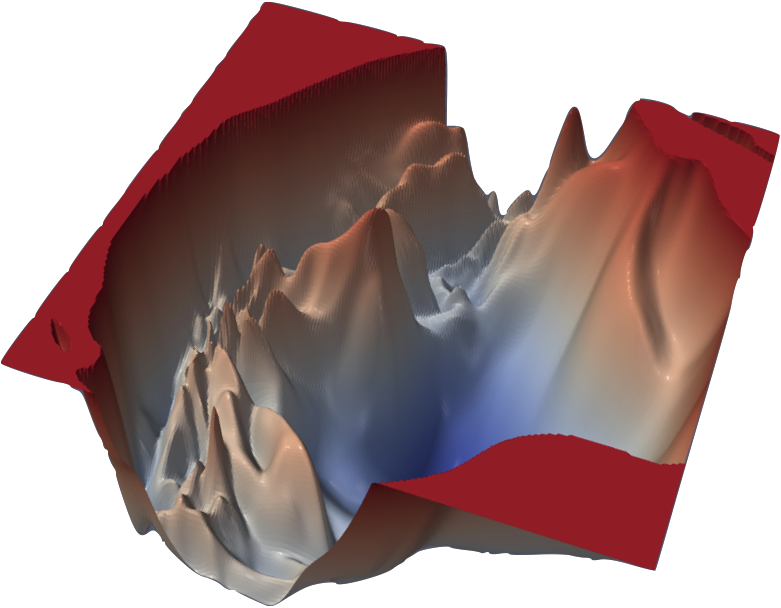
\includegraphics[width=0.3\textwidth]{losslandscape.png}
        \caption*{Possible loss landscape}
    \end{figure}
\end{frame}

\begin{frame}{Data Drift}
    \begin{definitionblock}{Definition}
        \begin{itemize}
            \item <1-> Covariate shift: distribution of the input variables $p(\mathbf{x})$ changes after deploying the model. Classes are not modified.
            \item <2-> Concept drift: conditional distribution $p(y|\mathbf{x})$ changes after deploying the model:
            \begin{enumerate}
                \item <3-> inputs previously assigned to one class may change label;
                \item <4-> new classes may altogether be formed.
            \end{enumerate}
        \end{itemize}
    \end{definitionblock}

    %\onslide<1->\begin{figure}
    %    \begin{tikzpicture}[xscale=0.5, yscale=1.5]
    %        \draw[->] (0.7,0.8) -- (2.3,0.8) node[below right] {};
            % Draw x-axis
    %        \draw[->] (-3,0) -- (6,0) node[below right] {$x$};
            % Draw first Gaussian function
    %        \draw[domain=-2.5:2.5,smooth,variable=\x,blue] plot ({\x},{exp(-\x*\x)});
            % Draw second Gaussian function
    %        \draw[domain=-2.5:2.5,smooth,variable=\x,red] plot ({\x+3},{exp(-\x*\x)});
    %    \end{tikzpicture}
    %    \caption*{Covariate shift}
    %\end{figure}
\end{frame}

\begin{frame}{Open-Set Recognition}
    \begin{definitionblock}{Definition}
        \begin{itemize}
            \item <1-> Open-set recognition (OSR): field of ML that assumes an incomplete knowledge of the world during training time.
        \end{itemize}
    \end{definitionblock}
    \begin{figure}[h]
        \scalebox{.68}{
            \begin{subfigure}{0.48\textwidth}
                \centering
                \begin{tikzpicture}
              
                  \pgfplotsset{
                      scale only axis,
                  }
              
                  \begin{axis}[
                    xmin=0, 
                    xmax=1.4, 
                    ymin=0, 
                    ymax=1.4,
                    %axis equal image
                    x=4.3cm,
                    y=4.3cm,
                    ticks=none]
                    \addplot [draw=customred,fill=customred, opacity=0.2]
                        coordinates {(0.65,0.7) (1.4,1.4) (1.4,0) (0.65,0)};
                    \addplot [draw=customgreen,fill=customgreen, opacity=0.2]
                        coordinates {(0.65,0.7) (0,1.4) (0,0) (0.65,0)}; 
                    \addplot [draw=customblue,fill=customblue, opacity=0.2]
                        coordinates {(0.65,0.7) (0.65,0.7) (1.4,1.4) (0,1.4)};
                    
                    \addplot[only marks, mark=x, color=black]
                    coordinates{
                      (0.61,0.72)
                      (0.63,0.75)
                      (0.67,0.69)
                      (0.62,0.64)
                      (0.65,0.65)
                      (0.63,0.68)
                      (0.63,0.7)
              
                      (1.21,0.07)
                      (1.23,0.13)
                      (1.27,0.15)
                      (1.22,0.1)
                      (1.25,0.19)
                      (1.3,0.1)
                      (1.3,0.2)
              
                      (1.21,1.37)
                      (1.23,1.33)
                      (1.27,1.35)
                      (1.22,1.21)
                      (1.25,1.29)
                      (1.3,1.31)
                      (1.3,1.25)
                    };
              
                    \addlegendimage{/pgfplots/refstyle=plot_one_1}
                    %\addlegendentry{plot 1}
              
                    \addplot[only marks, mark=+, color=customgreen]
                    coordinates{
                      (0.51,0.58)
                      (0.52,0.57)
                      (0.50,0.57)
                      (0.55,0.55)
                      (0.5,0.6)
                      (0.53,0.65)
                      (0.45,0.62)
                      (0.49,0.6)
                    };
                    
                    \addlegendimage{/pgfplots/refstyle=plot_two_1}
                    %\addlegendentry{plot 2}
              
                    \addplot[only marks, mark=asterisk, color=customblue]
                    coordinates{
                      (0.7,0.9)
                      (0.65,0.87)
                      (0.66,0.89)
                      (0.75,0.95)
                      (0.72,0.98)
                      (0.64,0.82)
                    };
                    \addlegendimage{/pgfplots/refstyle=plot_three_1}
              
                    \addplot[only marks, mark=o, color=customred]
                    coordinates{
                      (0.81,0.59)
                      (0.80,0.57)
                      (0.88,0.57)
                      (0.84,0.60)
                      (0.79,0.61)
                      (0.9,0.6)
                      (0.85,0.63)
                      (0.93,0.66)
                      (0.92,0.59)
                      % more points...
                    };
              
                    % plot 1 legend entry
                    \addlegendimage{/pgfplots/refstyle=plot_four_1}
                    %\addlegendentry{plot 2}
                    \node[] at (axis cs: 0.1,1.3) {$\mathcal{X}$};
                  \end{axis}
                \end{tikzpicture}
                \caption*{\Large{Closed-set recognition}}
                \end{subfigure}
                \qquad
                \begin{subfigure}{0.48\textwidth}
                \centering
                \begin{tikzpicture}
              
                \pgfplotsset{
                    scale only axis,
                }
                
                \begin{axis}[
                  xmin=0, 
                  xmax=1.4, 
                  ymin=0, 
                  ymax=1.4,
                  %axis equal image
                  x=4.3cm,
                  y=4.3cm,
                  ticks=none]
                 
              
                  \addplot[only marks, mark=x, color=black]
                  coordinates{
                    (0.61,0.72)
                    (0.63,0.75)
                    (0.67,0.69)
                    (0.62,0.64)
                    (0.65,0.65)
                    (0.63,0.68)
                    (0.63,0.7)
              
                    (1.21,0.07)
                    (1.23,0.13)
                    (1.27,0.15)
                    (1.22,0.1)
                    (1.25,0.19)
                    (1.3,0.1)
                    (1.3,0.2)
              
                    (1.21,1.37)
                    (1.23,1.33)
                    (1.27,1.35)
                    (1.22,1.21)
                    (1.25,1.29)
                    (1.3,1.31)
                    (1.3,1.25)
                  };
              
                  \addlegendimage{/pgfplots/refstyle=plot_one_2}
                  %\addlegendentry{plot 1}
              
                  \draw[rotate around={45:(0.51,0.60)},customgreen, fill=customgreen, fill opacity=0.2] (0.51,0.60) ellipse (10pt and 14pt);
                  \addplot[only marks, mark=+, color=customgreen]
                  coordinates{
                    (0.51,0.58)
                    (0.52,0.57)
                    (0.50,0.57)
                    (0.55,0.55)
                    (0.5,0.6)
                    (0.53,0.65)
                    (0.45,0.62)
                    (0.49,0.6)
                  };
              
                  
                  \addlegendimage{/pgfplots/refstyle=plot_two_2}
                  %\addlegendentry{plot 2}
              
                  \draw[rotate around={-35:(0.7,0.9)},customblue, fill=customblue, fill opacity=0.2] (0.7,0.9) ellipse (9pt and 15pt);
                  \addplot[only marks, mark=asterisk, color=customblue]
                  coordinates{
                    (0.7,0.9)
                    (0.65,0.87)
                    (0.66,0.89)
                    (0.75,0.95)
                    (0.72,0.98)
                    (0.64,0.82)
                  }; 
                  \addlegendimage{/pgfplots/refstyle=plot_three_2}
              
                  \draw[rotate around={-65:(0.87,0.61)},customred, fill=customred, fill opacity=0.2] (0.87,0.61) ellipse (9pt and 16pt);
                  \addplot[only marks, mark=o, color=customred]
                  coordinates{
                    (0.81,0.59)
                    (0.80,0.57)
                    (0.88,0.57)
                    (0.84,0.60)
                    (0.79,0.61)
                    (0.9,0.6)
                    (0.85,0.63)
                    (0.93,0.66)
                    (0.92,0.59)
                  }; 
              
                  % plot 1 legend entry
                  \addlegendimage{/pgfplots/refstyle=plot_four_2}
                  \draw[rotate around={0:(1.25,1.29)},black, fill=black, fill opacity=0.1] (1.25,1.29) ellipse (11pt and 16pt);
                  \draw[rotate around={-10:(1.26,0.13)},black, fill=black, fill opacity=0.1] (1.26,0.13) ellipse (10pt and 13pt);
                  \draw[rotate around={0:(0.64,0.7)},black, fill=black, fill opacity=0.1] (0.64,0.7) ellipse (8pt and 10pt);
                  
                  \node[] at (axis cs: 0.1,1.3) {$\mathcal{X}$};
                  \node[] at (axis cs: 0.6,1) {$S_1$};
                  \node[] at (axis cs: 0.38,0.7) {$S_2$};
                  \node[] at (axis cs: 1,0.72) {$S_3$};
                  \node[] at (axis cs: 0.53,0.75) {$U_1$};
                  \node[] at (axis cs: 1.1,1.25) {$U_2$};
                  \node[] at (axis cs: 1.2,0.3) {$U_3$};
              
                \end{axis}
                \end{tikzpicture}
                \caption*{\Large{Open-set recognition}}
            \end{subfigure}
        }
    \end{figure}
\end{frame}

\begin{frame}{Open-Set Recognition}
    \begin{normalblock}{Open-set recognition aim}
        \begin{itemize}
            \item Given input $\mathbf{x}_i$, aim is to: \begin{enumerate}
                \item <2-> predict if its label is \emph{known}:
                \[
                    \mathbf{y}_i \in \mathcal{K};
                \]
                \item <3-> correctly classify it.
            \end{enumerate}
            \item <4-> Training process: minimize \emph{expected error}:
            \[
                \mathcal{R} = \mathcal{R}_{\epsilon} + \alpha \mathcal{R}_{\mathcal{O}}\,.
            \]
        \end{itemize}
    \end{normalblock}
\end{frame}

\begin{frame}{Open-Set Risk}
    \begin{minipage}{0.55\textwidth}
        \begin{definitionblock}{Definitions}
            \begin{itemize}
                \item <1-> Embedding space of class $k$: 
                \[
                    \mathcal{S}_k \subset \mathcal{X}\,.
                \]
                \item <2-> Open space of class $k$:
                \[
                    \mathcal{O}_k = \mathcal{X}/\mathcal{S}_k = \mathcal{O}_k^{pos} \cup \mathcal{O}_k^{neg}\,.
                \]
            \end{itemize}
        \end{definitionblock}
    \end{minipage}%
    \begin{minipage}{0.45\textwidth}
        \onslide<1->\begin{figure}[h]
            \scalebox{.68}{
                \begin{tikzpicture}
    
                    \pgfplotsset{
                        scale only axis,
                    }
                    
                    \begin{axis}[
                        xmin=0, 
                        xmax=1.4, 
                        ymin=0, 
                        ymax=1.4,
                        %axis equal image
                        x=4.3cm,
                        y=4.3cm,
                        ticks=none]
                        
                    
                        \addplot[only marks, mark=x, color=black]
                        coordinates{
                        (0.61,0.72)
                        (0.63,0.75)
                        (0.67,0.69)
                        (0.62,0.64)
                        (0.65,0.65)
                        (0.63,0.68)
                        (0.63,0.7)
                    
                        (1.21,0.07)
                        (1.23,0.13)
                        (1.27,0.15)
                        (1.22,0.1)
                        (1.25,0.19)
                        (1.3,0.1)
                        (1.3,0.2)
                    
                        (1.21,1.37)
                        (1.23,1.33)
                        (1.27,1.35)
                        (1.22,1.21)
                        (1.25,1.29)
                        (1.3,1.31)
                        (1.3,1.25)
                        };
                    
                        \addlegendimage{/pgfplots/refstyle=plot_one_0}
                    
                        \draw[rotate around={45:(0.51,0.60)},customorange, fill=customorange, fill opacity=0.2] (0.51,0.60) ellipse (10pt and 14pt);
                        \addplot[only marks, mark=+, color=customorange]
                        coordinates{
                        (0.51,0.58)
                        (0.52,0.57)
                        (0.50,0.57)
                        (0.55,0.55)
                        (0.5,0.6)
                        (0.53,0.65)
                        (0.45,0.62)
                        (0.49,0.6)
                        }; 
                    
                        
                        \addlegendimage{/pgfplots/refstyle=plot_two_0}
                        %\addlegendentry{plot 2}
                    
                        \draw[rotate around={-35:(0.7,0.9)},customblue, fill=customblue, fill opacity=0.2] (0.7,0.9) ellipse (9pt and 15pt);
                        \addplot[only marks, mark=asterisk, color=customblue]
                        coordinates{
                        (0.7,0.9)
                        (0.65,0.87)
                        (0.66,0.89)
                        (0.75,0.95)
                        (0.72,0.98)
                        (0.64,0.82)
                        }; 
                        \addlegendimage{/pgfplots/refstyle=plot_three_0}
                    
                        \draw[rotate around={-65:(0.87,0.61)},customorange, fill=customorange, fill opacity=0.2] (0.87,0.61) ellipse (9pt and 16pt);
                        \addplot[only marks, mark=o, color=customorange]
                        coordinates{
                        (0.81,0.59)
                        (0.80,0.57)
                        (0.88,0.57)
                        (0.84,0.60)
                        (0.79,0.61)
                        (0.9,0.6)
                        (0.85,0.63)
                        (0.93,0.66)
                        (0.92,0.59)
                        % more points...
                        };
                    
                        % plot 1 legend entry
                        \addlegendimage{/pgfplots/refstyle=plot_four_0}
                        
                        \node[] at (axis cs: 0.15,1.3) {$O^{neg}_1$};
                        \node[] at (axis cs: 0.6,1) {$S_1$};
                        \node[] at (axis cs: 0.38,0.72) {$O^{pos}_1$};
                        \node[] at (axis cs: 1,0.74) {$O^{pos}_1$};
                    
                    \end{axis}
                \end{tikzpicture}
            }
            \caption*{Subdivision of $\mathcal{X}$}
        \end{figure}
    \end{minipage}
\end{frame}

\begin{frame}{Open-Set Risk}
    \begin{definitionblock}{Definitions}
        \begin{itemize}
            \item <1-> Recognition function: 
            $\phi_k: \mathcal{X} \to \{0,1\}$ such that:
            \[
                \phi_k = \begin{cases}
                1 & \text{if $\mathbf{x}$ is classified as \emph{k}}, \\
                0 & \text{otherwise}.
                \end{cases}
            \]
            \item <2-> Open space risk for class $k$:
            \[
                \mathcal{R}_{\mathcal{O}}(\phi_k, \mathcal{O}^{neg}_k) = \frac{\int \limits_{\mathcal{O}^{neg}_k} \phi_k(x)dx}{\int \limits_{\mathcal{X}} \phi_k(x)dx}.
            \]
        \end{itemize}
    \end{definitionblock}
\end{frame}